\chapter{3D打印建模}
\label{cha:Model}

\section{测试用3轮底盘}

需要考虑到电机和定位模块的配合。

定位模块外形为 $\phi$ 11.2 X 25.1mm,至少需要留12mm直径的圆柱形空间,头部距离地面不得超过2mm。定位模块外形尺寸如图~\ref{fig:Camera-Dimension}。

\begin{figure}[htbp]
    \centering
    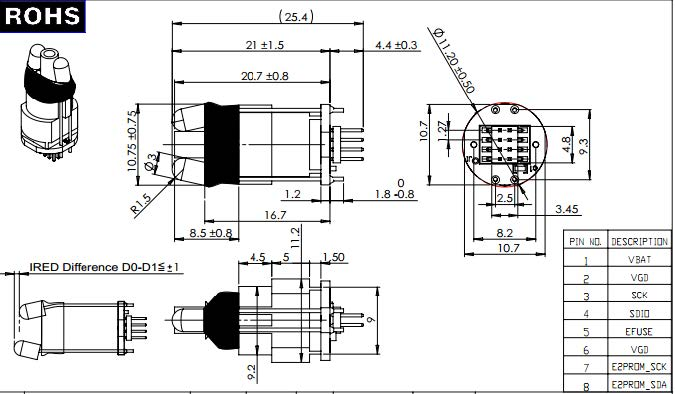
\includegraphics[width=\columnwidth]{SONIX_OID_SNM9S500C3000A_Specification_V1-Dimension.jpg}
    \caption{定位模块外形尺寸}
    \label{fig:Camera-Dimension}
\end{figure}

定位模块配套母排离PCB高度为4.3mm,所以Camera下端居PCB底面约为27mm,根据经验需要预留7-10mm的离地距离,所以按照35mm预留,小于轮子直径38mm,考虑可以加一个延长针脚座使用,所以PCB离地设计为50mm。


底盘装配图如图~\ref{fig:Assembled-Test-Datasheet}。

\begin{figure}[htbp]
    \centering
    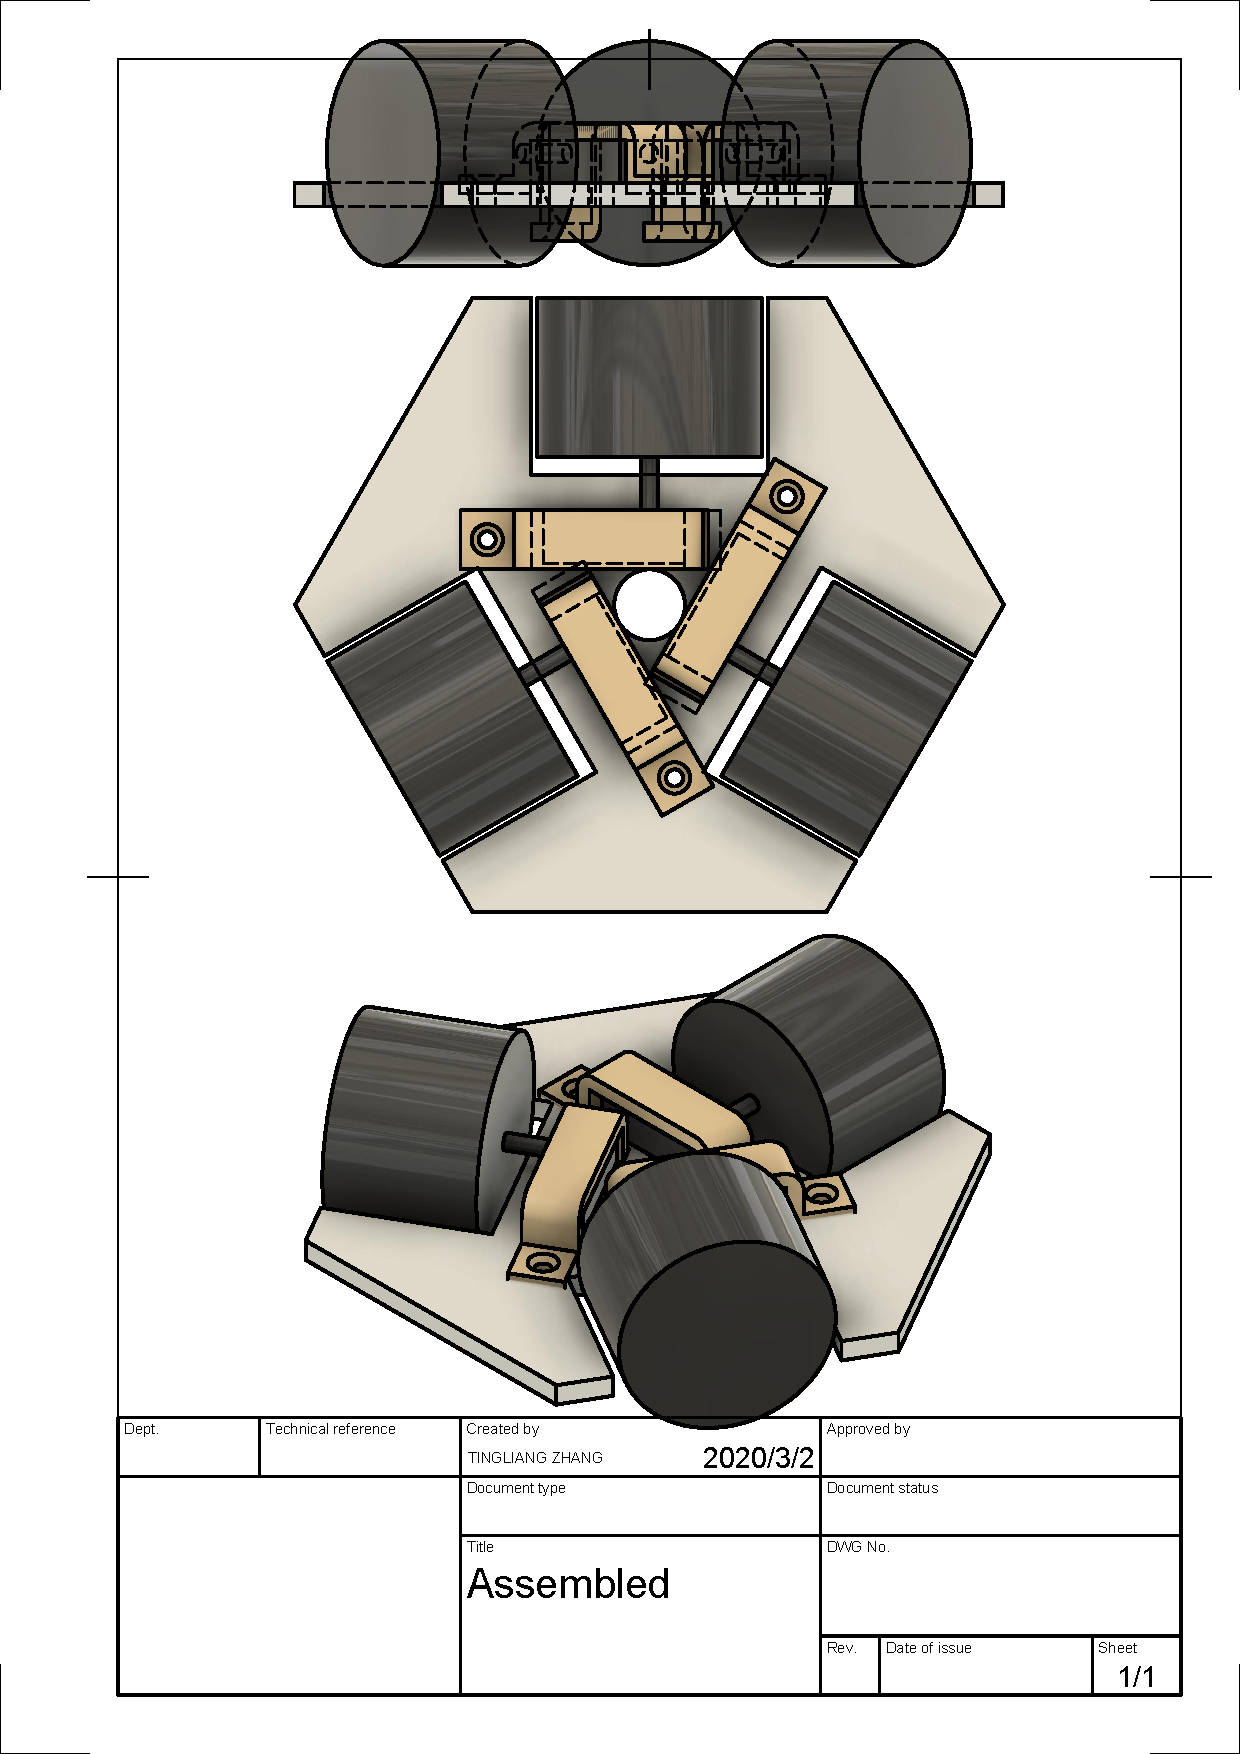
\includegraphics[width=\columnwidth]{Assembled-v1.pdf}
    \caption{测试用底盘装配图}
    \label{fig:Assembled-Test-Datasheet}
\end{figure}

测试用底盘渲染图如图~\ref{fig:Assembled-Test-Render}。

\begin{figure}[htbp]
    \centering
    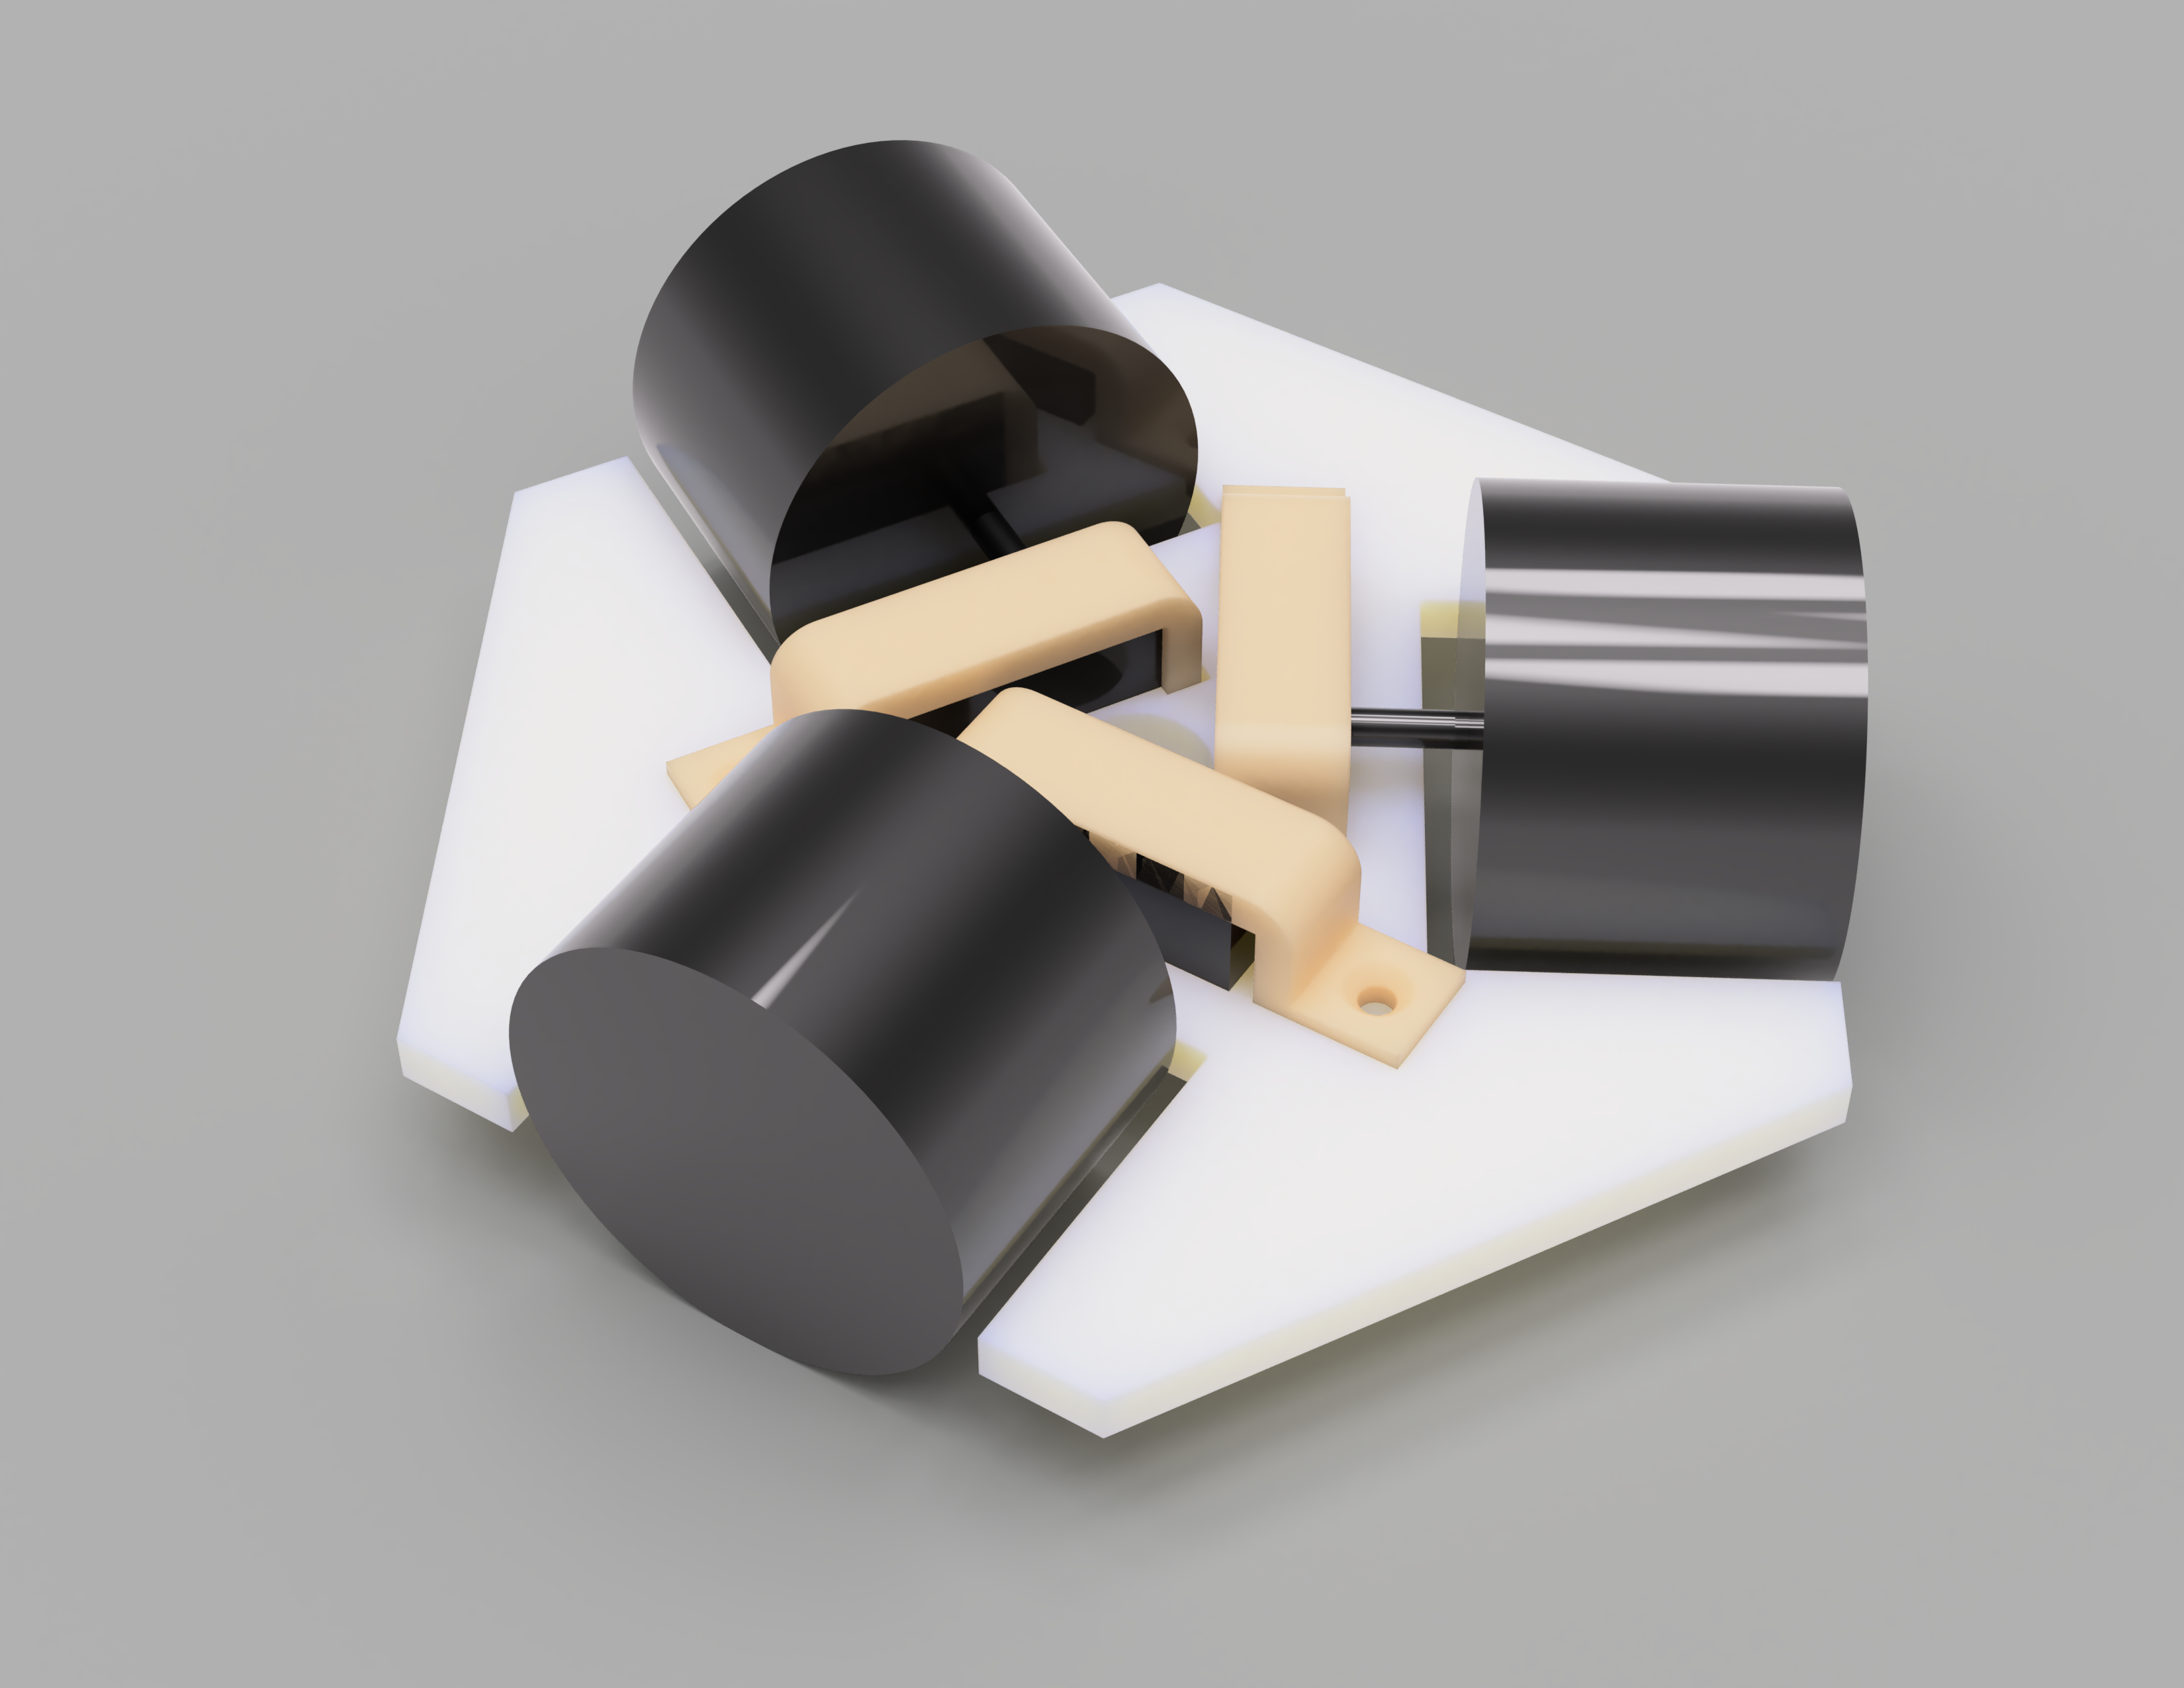
\includegraphics[width=\columnwidth]{Assembled_2020-Mar-02.png}
    \caption{测试用底盘渲染图}
    \label{fig:Assembled-Test-Render}
\end{figure}

其中,电机固定件使用的是一颗沉头M3*10的不锈钢螺栓。固定件上留出大径5.3mm小径3mm的沉头螺丝孔,底板上则留一个直径5.9mm圆内接正六边形深度为2.5mm的六角螺母固定孔,以便不用鸭嘴钳拧螺丝,当然也有3mm的圆孔。如图~\ref{fig:BottomTest-v1-Datasheet}和图~\ref{fig:StepperMount-v1-Datasheet}。

\begin{figure}[htbp]
    \centering
    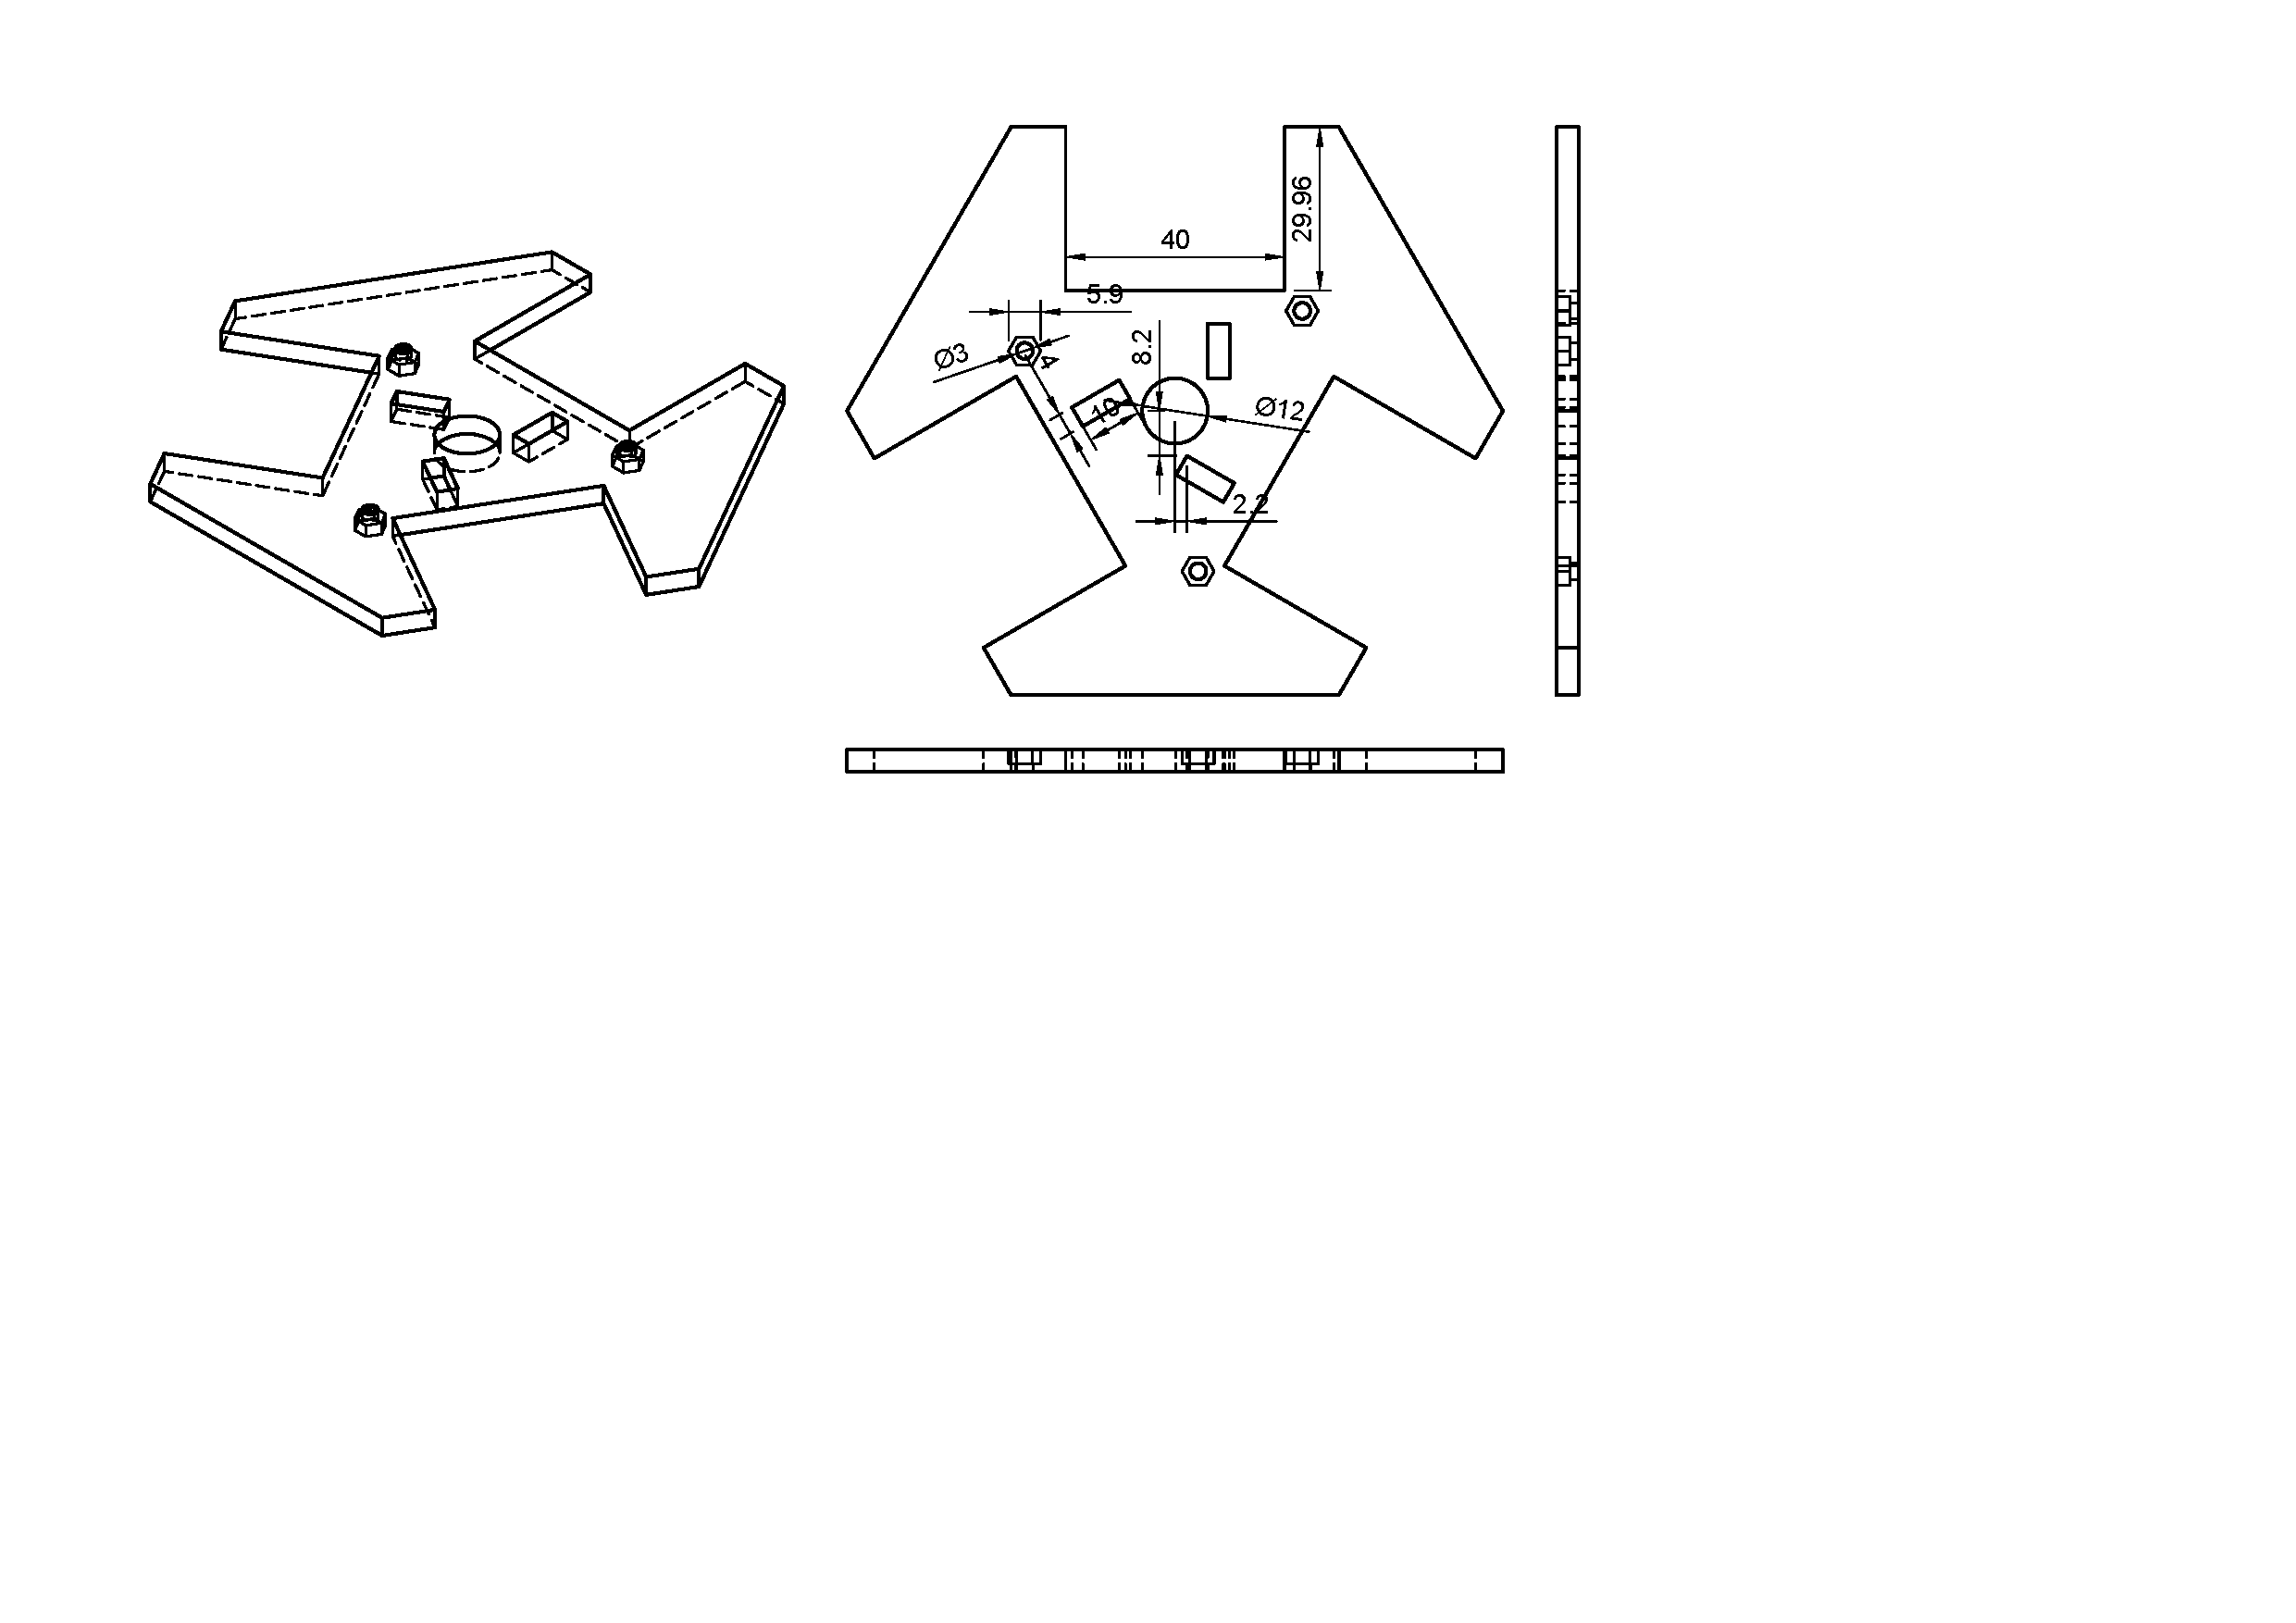
\includegraphics[width=\columnwidth]{BottomTest-v1.pdf}
    \caption{测试用底盘图纸}
    \label{fig:BottomTest-v1-Datasheet}
\end{figure}

由于两电机之间间隙(矩形可延展4.39mm)不足以放下一个M3螺丝,所以采用了一边卡扣的形式来固定。

\begin{figure}[htbp]
    \centering
    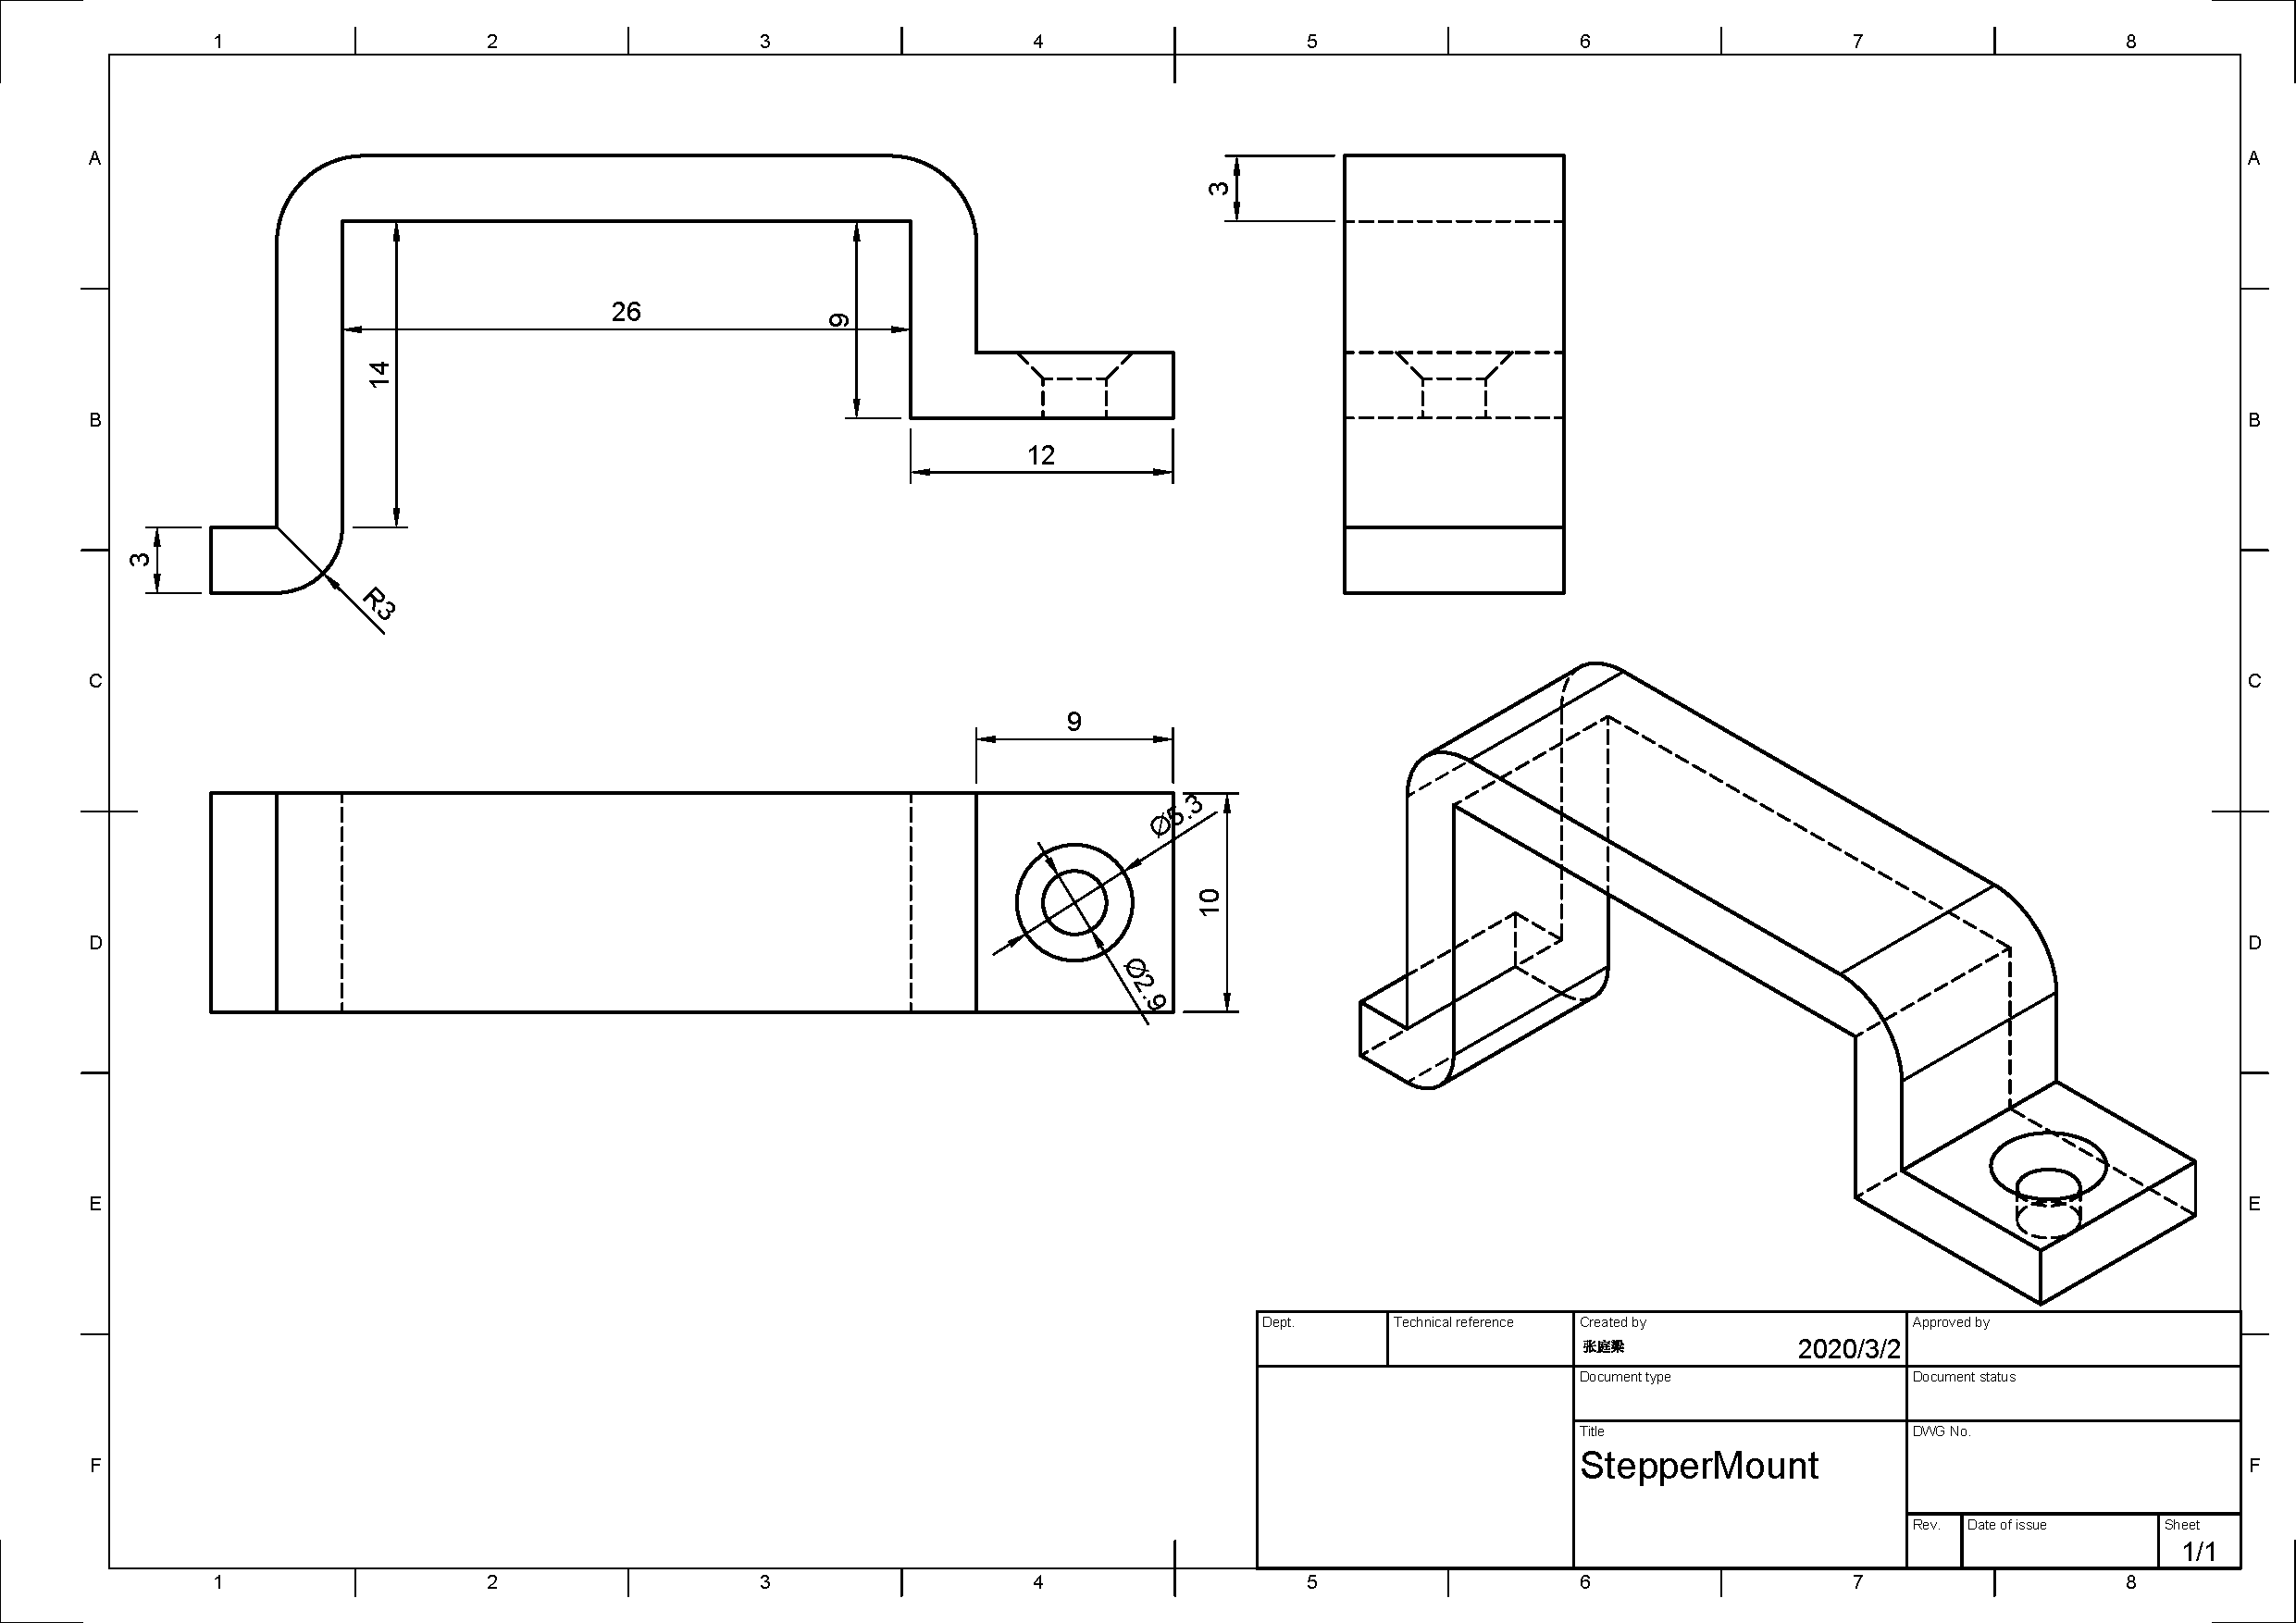
\includegraphics[width=\columnwidth]{StepperMount-v1.pdf}
    \caption{步进电机固定座图纸}
    \label{fig:StepperMount-v1-Datasheet}
\end{figure}

其中步进和轮子画为一个零件,作确定装配体尺寸用,如图~\ref{fig:StepperAndWheel-v0-Datasheet}。

\begin{figure}[htbp]
    \centering
    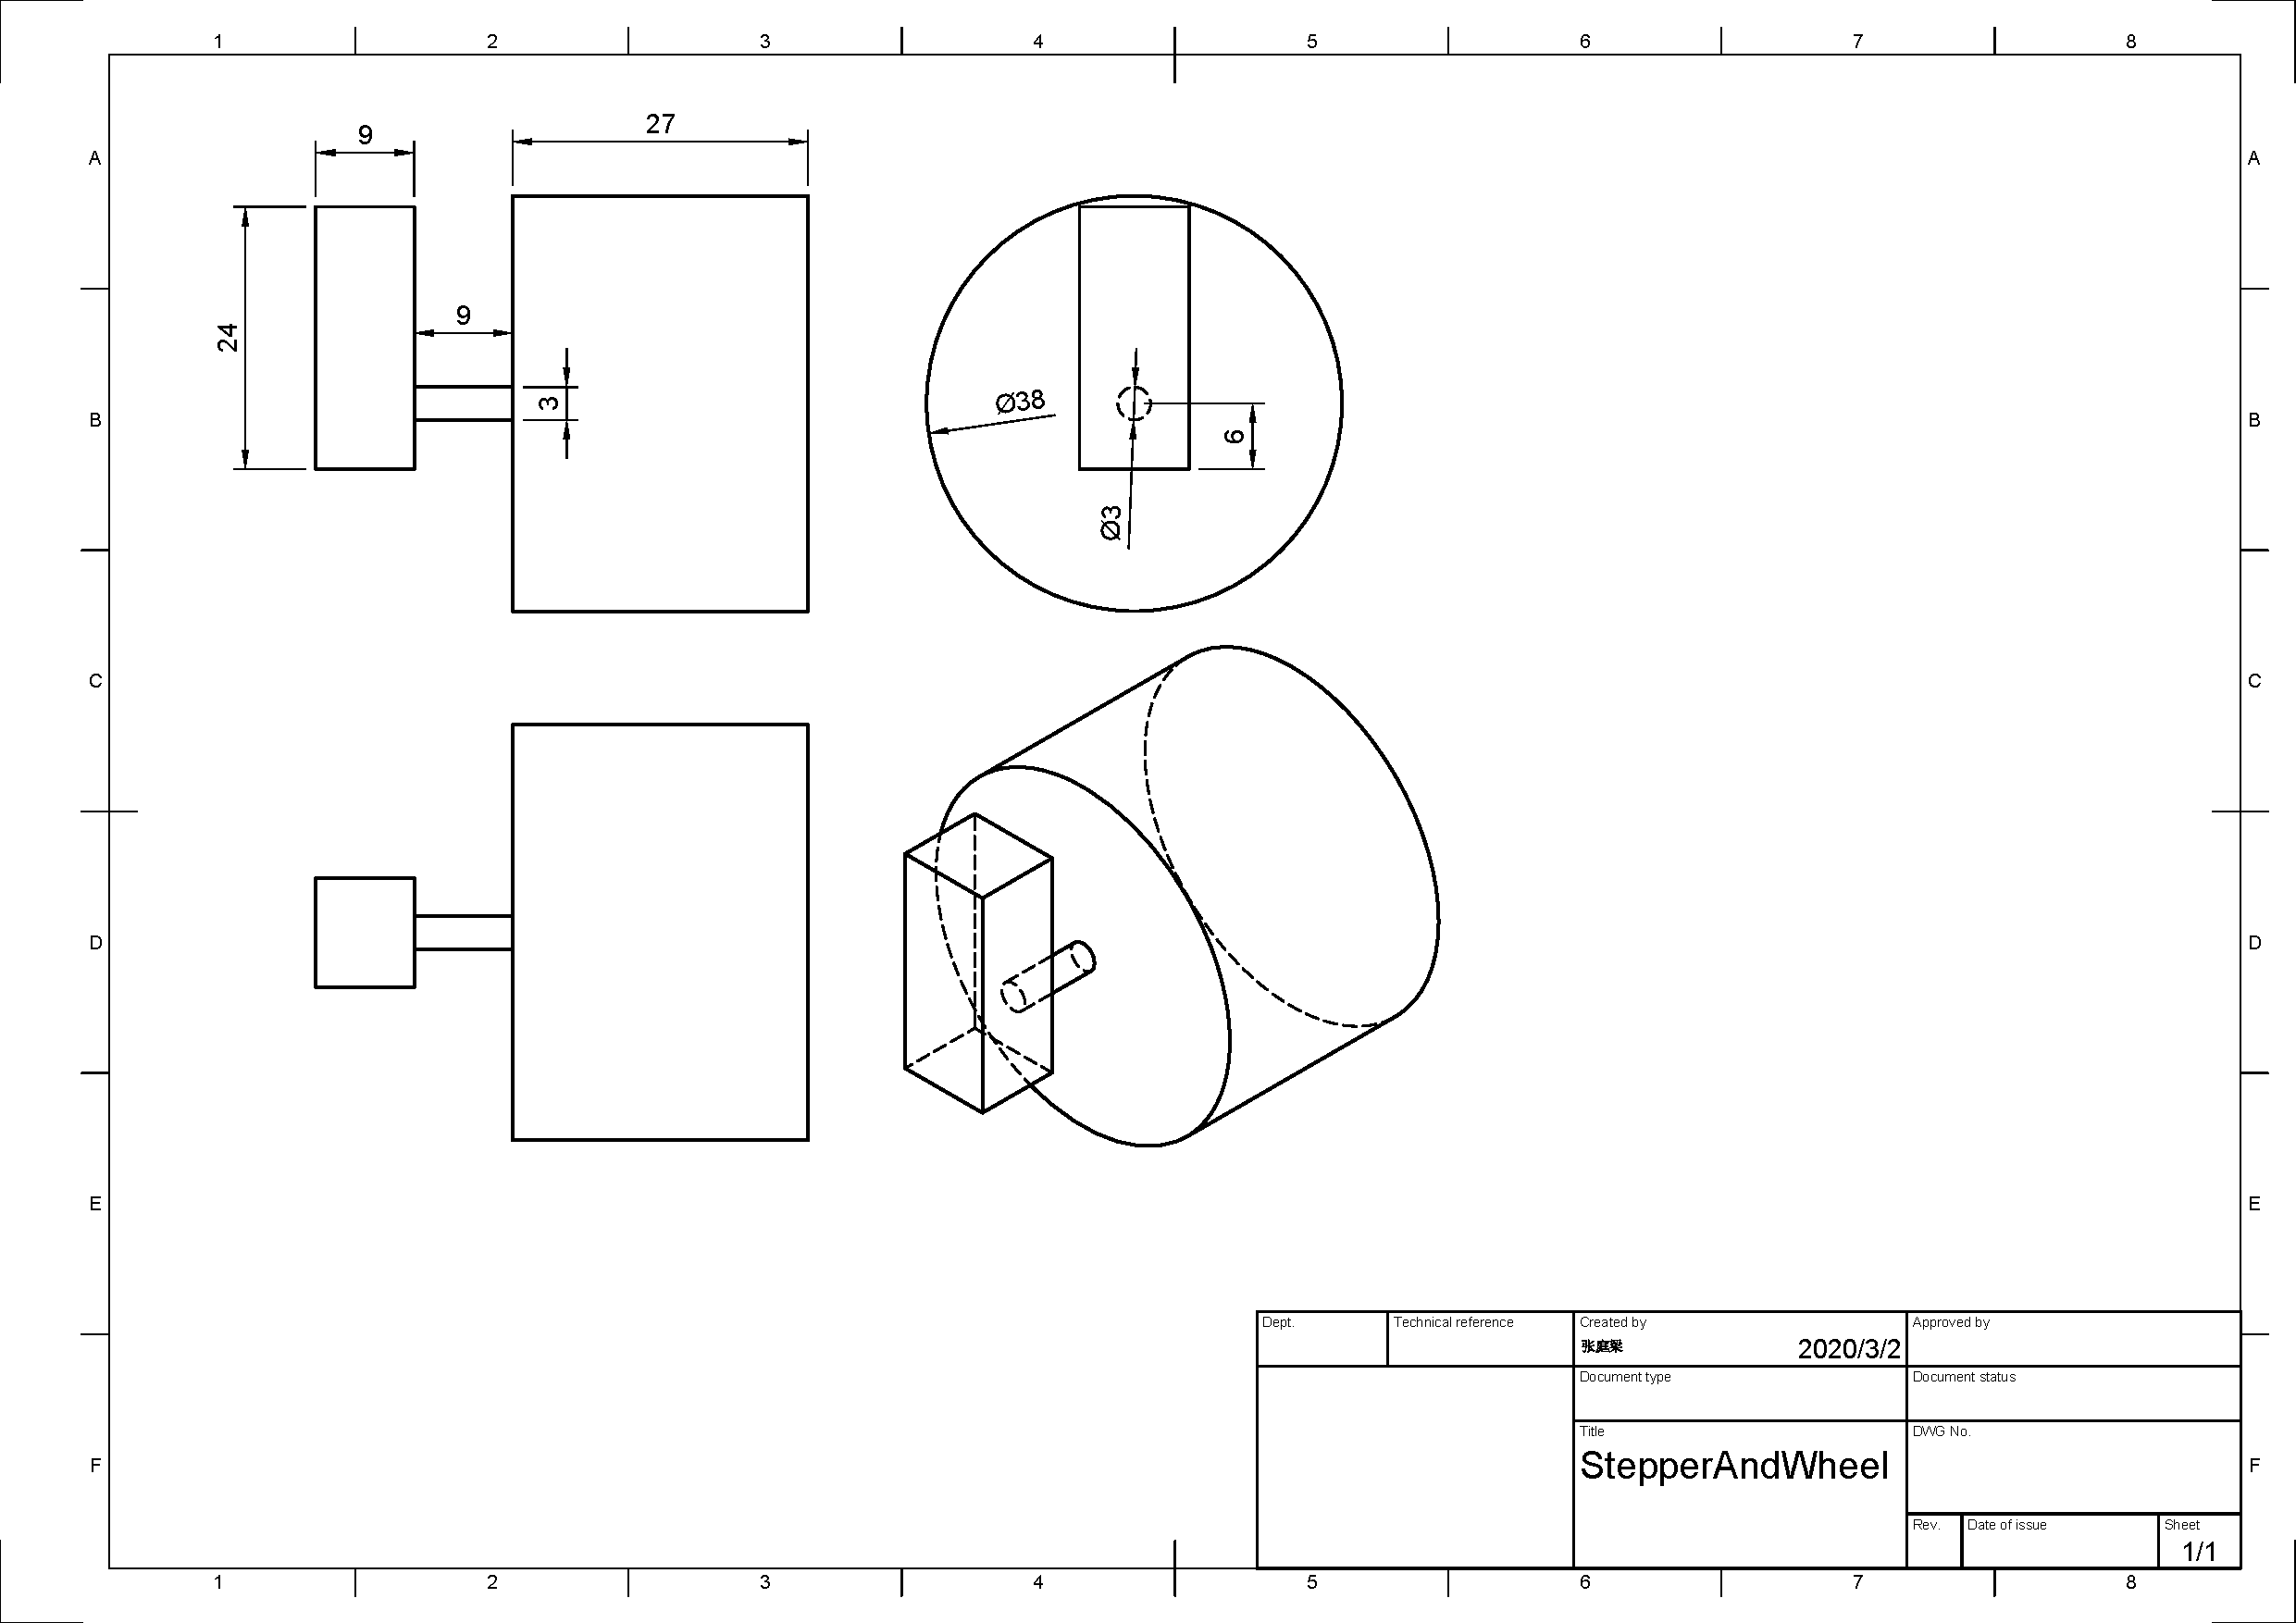
\includegraphics[width=\columnwidth]{StepperAndWheel-v0.pdf}
    \caption{步进和轮子图纸}
    \label{fig:StepperAndWheel-v0-Datasheet}
\end{figure}


电机固定加凹槽,固定一下前后位置。

PCB放置到凹槽里面,固定水平位置

电机固定一颗螺丝固定相邻两个电机,重叠边沿打孔。


\section{关键参数计算}

